\documentclass{article}
\usepackage[utf8]{inputenc}
\usepackage{lstautogobble}
\usepackage[export]{adjustbox}
\usepackage{graphicx}
\usepackage{changepage}
\usepackage{listings}
\usepackage{amsthm}
\usepackage{subcaption}
\usepackage{amssymb}

\lstset{ %
  language=Promela,                  % the language of the code
  basicstyle=\footnotesize,       % the size of the fonts that are used for the code
  numbers=left,                   % where to put the line-numbers
  numberstyle=\tiny\color{gray},  % the style that is used for the line-numbers
  stepnumber=1,                   % the step between two line-numbers. If it's 1, each line 
                                  % will be numbered
  numbersep=5pt,                  % how far the line-numbers are from the code
  backgroundcolor=\color{white},  % choose the background color. You must add \usepackage{color}
  showspaces=false,               % show spaces adding particular underscores
  showstringspaces=false,         % underline spaces within strings
  showtabs=false,                 % show tabs within strings adding particular underscores
  frame=single,                   % adds a frame around the code
  rulecolor=\color{black},        % if not set, the frame-color may be changed on line-breaks within not-black text (e.g. commens (green here))
  tabsize=4,                      % sets default tabsize to 2 spaces
  captionpos=b,                   % sets the caption-position to bottom
  breaklines=true,                % sets automatic line breaking
  breakatwhitespace=false,        % sets if automatic breaks should only happen at whitespace
  title=\lstname,                 % show the filename of files included with \lstinputlisting;
                                  % also try caption instead of title
  keywordstyle=\color{blue},          % keyword style
  commentstyle=\color{dkgreen},       % comment style
  stringstyle=\color{mauve},         % string literal style
  escapeinside={\%*}{*)},            % if you want to add a comment within your code
  morekeywords={*,...}               % if you want to add more keywords to the set
}

% the following is needed for syntax highlighting
\usepackage{color}

\definecolor{dkgreen}{rgb}{0,0.6,0}
\definecolor{gray}{rgb}{0.5,0.5,0.5}
\definecolor{mauve}{rgb}{0.58,0,0.82}

\renewcommand{\phi}{\varphi}
\newcommand{\always}{\Box}
\newcommand{\eventually}{\Diamond}
\newcommand{\calL}{{\cal L}}
\newcommand{\until}{\; {\cal U} \;}
\newcommand{\neXt}{{\cal X} \;}
\newcommand{\implies}{\rightarrow}
\newcommand{\allpaths}{\; {\cal A} \;}
\newcommand{\existspath}{\; {\cal E} \;}

\begin{document}

\title{Applying Formal Techniques\\ to Solving Rubik's Cubes\\[3cm] SatRubiks }

\author{Nathan Scheirer, Joshua Wallin, Patrick Sivets}

\maketitle
\newpage

\section{Introduction}
At some point in life the question has had to have come up; how can I solve a Rubik's cube? For some of us that takes a lot of practice and studying of various algorithms to solve any scrambled cube that's given to us. However, for the rest of us, who don't have time to learn all these different algorithms, yet still want the satisfaction of solving the most popular toy ever created there must be an easier way. That's where the concept of solving a Rubik's cube with formal methods comes into play. How nice would it be to be able to just input the starting condition of the cube into your solver and have a sequence of moves spit back out that exactly solves your puzzle? In our opinion, that would be very nice. So in this study we take a look at a few various formal method solvers to see if this application is feasible and, if so, which is the best method to use. 

\section{Spin Model Checker}
\subsection{Background}
The SPIN Model Checker was developed in the early 1980s at Bell Labs and has been freely available for use since 1991. SPIN is a popular verification tool using the Promela (Protocol Meta Language) language. However, Spin has not been used in conjuncture with solving puzzles. Upon researching Spin it was only seen in one piece of literature where Spin was used as a puzzle solver. In the paper \textit{Spin for puzzles: Using Spin for solving the Japanese river puzzle and the Square-1 cube} by Evgeny V. Bodin et al., they use Spin to model and solve common puzzles with the use of planning. Spin can be used in a very similar manner to solve the 2x2 Rubik's Cube.

\subsection{Set-Up}
\subsubsection{Initial Programs}
Correctly representing the Rubik's cube and its transitions in Promela proved to be a tricky task. Our initial attempts to create a working model lead to a long list of errors and rather inefficient code. The initial model had several places in the code where errors were present. First, there was an inconsistency with our description of the cube in Promela. The physical cube did not reflect what was encoded into our model. This oversight led to further errors including, misrepresentation of transitions and incorrect final states. To correct these fatal errors, a new model needed to be developed to accurately depict the 2x2 Rubik's cube.\\[3mm]
In order to achieve an accurate representation, a simple model was created to represent a ``two-sided'' cube. This is an idea where a cube only has two sides and where those sides are each a different color and the model must accurately swap these colors during a transition.  This ``two-sided'' cube was modeled using the code: 
\begin{verbatim}
byte a = 1, b = 0;

byte temp1 = 0;

#define FINISH ((a == 0) && (b == 1))

active proctype test()
{
	     do
	     ::  assert(!FINISH) -> atomic {
		          temp1 = a;
		          a = b;
		          b = temp1;
	         }
	     od
}

\end{verbatim}
In this code each side is represented using bytes a and b, which are both assigned a color using boolean values. To define the transition, a variable is defined to act as a temporary value store. Within the do-loop is where the transition occurs and by defining the transitions in this way, the model was able to accurately able to give a counter-example leading to the final state as defined in the code. \\[3mm]
The idea from this simple ``two-sided'' cube was extended to a normal six-sided cube with each face a different color. This model was very similar in how it was written, using variable to temporarily store the sides color information during the transitions. One main difference in this code is that there needed to be two different transitions represented, one in the vertical direction and one in the  horizontal. To do this it was defined that the horizontal direction would rotate clockwise and the vertical direction upwards. The code for the horizontal transition is shown below. 
\begin{verbatim}
byte a=1, b=2, c=3, d=4, e=5, f=6;
byte tmp1, tmp2, tmp3, tmp4, tmp5, tmp6, tmp7, tmp8;
#define FINA (a==4)
#define FINB (b==1)
#define FINC (c==2)
#define FIND (d==3)
#define FINE (e==5)
#define FINF (f==6)
#define FINAL (FINA && FINB && FINC && FIND && FINE && FINF)
active proctype test(){
	     do
	          :: assert(!FINAL)-> atomic{
		          printf("right");
		          tmp1=a;
				          tmp2=f;
		          tmp3=c;
		          tmp4=e;
		          f=tmp1;
		          c=tmp2;
		          e=tmp3;
		          a=tmp4
		          }
	    .
    .
    .

\end{verbatim}
An issue that this code brought to light is how to appropriately define the final state in Promela. As shown above that was done by using the define function and setting the final state of each side. This removed the need for long LTL properties and it kept the code clean and concise. To verify that this model represented the six-sided cube appropriately it had to be checked that the final state could actually exist. When running the code with an end state that did not exist the code would not give a trace stating how we could reach that state. 
\subsubsection{2x2 Rubik's Cube}
The same ideas that were used in the simple initial programs could be applied to the more complex 2x2 Rubik's Cube. However, in order to accurately represent the cube and its movements, the cube must be appropriately represented in Promela. To do this a system was implemented that labeled each ``face-let'' of the cube in accordance to its orientation. This is shown in the picture below. \\[7mm]
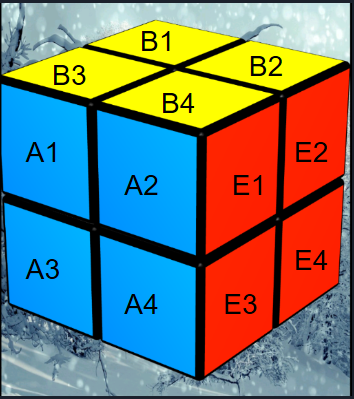
\includegraphics[width=.5\textwidth, center]{pics/Facelet.PNG} \\[7mm]
As shown in the picture, the 2x2 cube's face-lets were defined with each face receiving a designated letter (A-F) and that letter was paired with a number corresponding to the face-let position, with the number one beginning in the top left through four in the bottom left corner. It was also encoded to represent each color by an integer value. Labeling the cube in this consistent way allowed for the transitions to be reflected accurately. \\[3mm]
To accurately reflect these transitions it must be known that there are only six different moves that can be made with a standard 2x2 Rubik's Cube. \\[7mm]
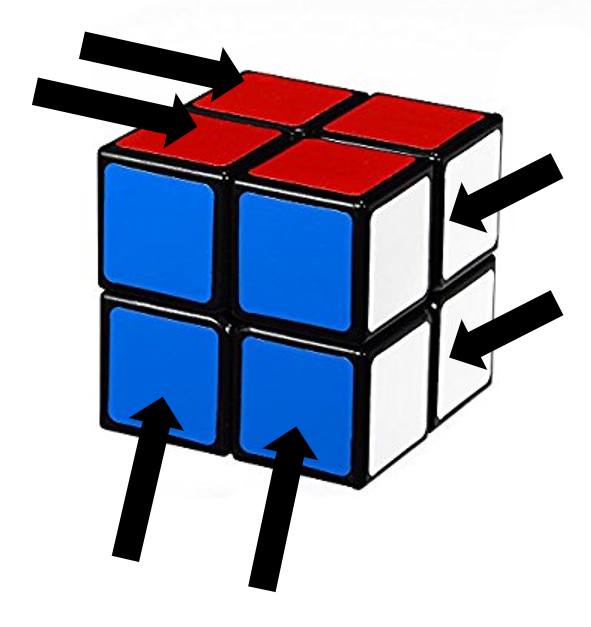
\includegraphics[width=.5\textwidth, center]{pics/Capture5} \\[7mm]
These moves, reflected above, were all set to rotate in a clockwise direction. Again, this consistency allowed for the encoded transitions to reflect the physical cube's movements. \\[3mm]
The final aspect of the cube that needed to be encoded was the final state that the program was attempting to reach. Initially, this proved to be a very messy and long LTL property due to the fact that each side could have six possible colors when the cube was solved. However, the SatRubiks team found that this issue could be cleaned up by working backwards. Meaning that instead of having an initial state be the random configuration of the cube, the initial state could be encoded to represent a solved cube and the final state would then represent the random configuration. This idea removed the need for nasty LTL properties and made made the code relatively easy to read and understand. \\[3mm]
Now that the cube has been setup accurately with Promela and the transitions have been correctly encoded, the ideas that were utilized in the initial programs are ready to be applied to the 2x2 Rubik's cube. The full Promela code for the 2x2 Rubik's cube can be found in Appendix B or on GitHub in the SatRubiks repository. \\[3mm]
It is important to note that when running this code with Spin some of the settings will have to be adjusted. For instance, when running this code the ``physical memory available'' will have to be adjusted from its default setting to that of at least 1,000,000 MB. If this setting is not adjusted it causes catastrophic errors within Spin and the program will fail to run. Another important aspect of running this code is that the search mode will need to be changed from depth-first search to breadth-first search. This will change the way that Spin searches the state-space of the cube. Instead of ``walking through'' each node one by one as it does in a depth search, Spin will search the node's nearest neighbors before moving on down the state-space tree. This significantly reduces run times. When run with the depth-first search set the program was seeing run times anywhere from 30 minutes to well over an hour. Changing this setting cut the run times down to the level of seconds to a few minutes. 
\subsection{Results}
In order to generate random configurations of a 2x2 Rubik's cube, the SatRubiks team used a popular application for the iPhone, \textit{Cube 3D Kit}. This application provided a platform that could not only generate random initial conditions but also allow the user to attempt to solve the puzzle. Using this application, several random configurations were generated and ran against the Spin model. Depending on the initial configuration of the cube the model could solve it in as little as half a second, however in some uncommon cases it could take up to a couple minutes. Below are two different configurations of the 2x2 cube that were checked against the model. \\

\begin{figure}[!h]
  \centering
  \begin{minipage}[b]{0.4\textwidth}
    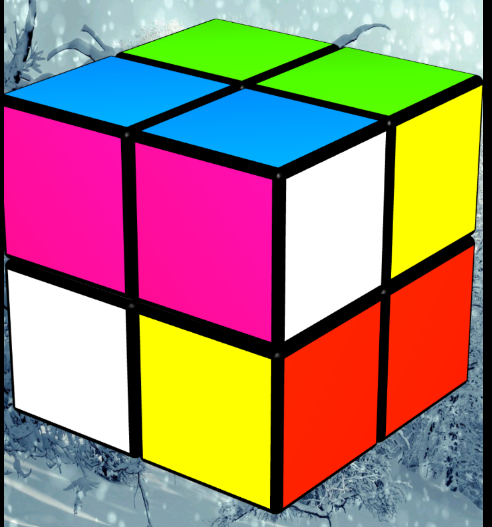
\includegraphics[width=\textwidth]{pics/Capture6.PNG}
    \caption{Random Config.A}
  \end{minipage}
  \hfill
  \begin{minipage}[b]{0.4\textwidth}
    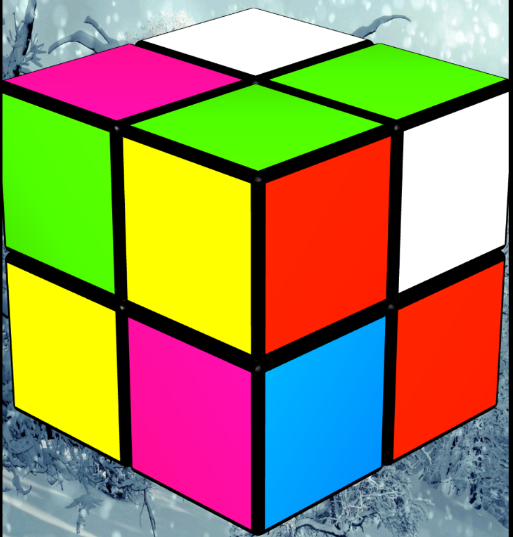
\includegraphics[width=\textwidth]{pics/Capture8.PNG}
    \caption{Random Config. B}
  \end{minipage}
\end{figure}
By inputting the appropriate orientation into the Spin model, the algorithm provided a correct path that led to the solved cube when followed in reverse. Note that each clockwise transition will now represent a counter-clockwise transition due the backward nature of the program. In the first case, the algorithm was able to solve the puzzle in just .49 seconds. Provided a path that consisted of seven moves to be solved.  The second configuration took a little longer for the algorithm to solve, solving it in 10.9 seconds. This amount of time was rather common when running other tests. Only in a few instances was there long run times of several minutes. However, there was not a lot of consistency in the run times and some instances where this model was not able to solve the initial configuration given.
\subsection{Verification and Future Work}
Attempting to make sure that the model accurately reflected the cube and its moves was one of the more difficult tasks. There was no real good way to validate the transitions aside form the use of inspection. To make this as accurate as possible, all transitions were explicitly written out including what each face-let was doing during a single rotation. These were then compared with the encoded information to ensure an that the physical cube was appropriately reflected. \\[3mm]
The model was also verified by using the way the cube is constructed and checking to see if certain configurations are allowed in the model. For instance, in the cube above yellow and white are on opposite sides of the cube and thus can never be next to each other in any configuration. By using simple LTL propositions, such as !(b3 == 2 \&\& a1 == 4) if two and four represent yellow and white receptively, this can be check to be sure that the model does 
not allow this to occur. This same principle can also be applied to trying to find paths that lead to impossible end states in our model. Running the model using a final state that represents white and yellow being next to each other the algorithm should not produce any trace that allows for this either. \\[3mm]
There is still more work needing to be done with the 2x2 model. The model should be able to solve every configuration that it is given. This could be a memory issue within Spin, it is not clear. However, expanding this model to the 3x3 cube should not be overly difficult considering how the 2x2 cube is represented and how the transitions are encoded.  The concern with this is with the memory limitations that were encountered using the Spin for the 2x2 model. 

\section{Pure SAT Solving}
\subsection{Background}
Satisfiability solving (SAT) is a method for determining the satisfying solution to a given boolean equation. SAT solving was the first problem to be determined NP-complete via the Cook-Levin theorem. Therefore, this formal method provides a unique and promising solution to the problem discussed in this paper, the Rubik's cube.
\subsection{Set-Up}
\subsubsection{Method}
In regards to solving a Rubik’s cube with formal methods, using a Satisfiability Solver (SAT) has been discussed the most throughout literature [1]. Therefore, this approach, initially, appeared to be the most straightforward of the processes discussed in this paper. This proved to be true as work started on developing the pure SAT model. With the aid of a program called Sabr [2], creating SAT queries for the Rubik’s cube became not only trivial but extremely simple. Not only were the models easy to develop but Sabr also parses the output of any given SAT solver into a format that is easy to read and follow. This allowed us to compare the efficiency of the Sabr parsing with that of NuXmv as well as the efficiency of a variety of SAT solving back ends. The overall process for solving a Rubik’s cube via SAT can be observed in figure 3: \\[7mm]
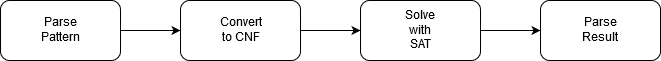
\includegraphics[width=1\textwidth, center]{pics/satfigure1.png} \\
\begin{center}
Figure 3. SAT Solving process \\[7mm]
\end{center}
\subsubsection{Parsing with Sabr}
This input to Sabr comprises of a few different main definitions: Board, Start, End, and DesObjs. With these components a model can be created as seen in model Appendix B. The initial state of an unsolved Rubik’s cube is placed in the Start definition with the following structure:\\[7mm]
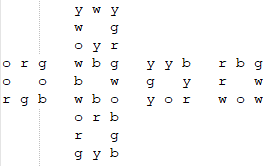
\includegraphics[width=0.5\textwidth, center]{pics/initialsabrmodel.PNG} \\
\begin{center}
Figure 4. Initial Sabr model condition \\[7mm]
\end{center}
Sabr then converts this initial condition, along with the transition definitions, into a SAT query that can be inputted into any SAT solver that utilizes the conjunctive normal form (CNF) formula structure. CNF is a form of logical equation that is constructed of ands of clauses of ors. An example of a CNF formula can be observed below where each new line is denoted with a 0 and each line is a new clause. Each variable can either be positive or negative, where negative numbers represent the negation of that variable. The first line of a CNF formula (starting with a “p”) expresses the number of variables and the number of clauses in the generated formula. These numbers were useful later in determining the correctness of the developed models because the number of variables used to solve a Rubik’s cube is known. \\
\begin{center}
p cnf 2484 23442 0 71 0 113 0 211 0 295 0 337 0 \hfill Equation 1
\end{center}
\subsubsection{SAT Solvers}
Two SAT solvers were considered during this project, the first being a SAT solver created during the 2017 SAT competition called CaDiCaL [3] and the second being the popular solver miniSat. MiniSat was chosen because of its popularity and it is also the back-end for NuXmv which allowed for another avenue of comparison between the proposed models. CaDiCaL was chosen for its performance in the agile track during the 2017 SAT solver competition. Placing first in this category showed that this was one of the quickest and simplest solvers created just recently. This created an interesting dimension to the comparison described throughout this paper.
\subsection{Results}
Initially, a 2x2 model of the Rubik’s cube was created to determine the feasibility of the proposed SAT method. What soon became obvious was that this method was very easy to work with and the results were proving to be accurate after a few test runs of the model. Only a few patterns that were tested resulted in long run times and were unable to be solved. Following the success of the 2x2 model a 3x3 model was created and analysis was performed on the results of that model as well. Unlike the 2x2 model, the 3x3 model proved to be much more difficult to get results, with most patterns running for days without a solution. This made it difficult to produce usable results from the 3x3 model, however the method was verified with the 2x2 model and the results from that are still very comparable to the other methods described in this paper.
\subsubsection{2x2 Model}
Average benchmarking results can be observed in table 1 below with extended results available in the Github source and in A1. \\
\begin{center}
Table 1. 2x2 Rubik's Cube average results \\
\begin{tabular}{|c|c|c|}
\hline
\multicolumn{3}{|c|}{2x2 Rubik's Cube} \\
\hline
& CPU Time (s) & Memory Used (Mb) \\
\hline
Sabr/miniSAT & 216.4 & 31.41 \\
\hline
CaDiCaL & 43.96* & 12.394 \\
\hline
\end{tabular} \\[0.1mm]
* Encountered runtimes $>$ 200,000 seconds
\end{center}

\subsubsection{3x3 Model}
Average benchmarking results can be observed in table 2 below with extended results available in the Github source and in A2. \\
\begin{center}
Table 2. 3x3 Rubik's Cube average results \\
\begin{tabular}{|c|c|c|}
\hline
\multicolumn{3}{|c|}{3x3 Rubik's Cube} \\
\hline
& CPU Time (s) & Memory Used (Mb) \\
\hline
Sabr/miniSAT & 5041.31 & 305.36 \\
\hline
CaDiCaL & NA & NA \\
\hline
\end{tabular}
\end{center}
\subsubsection{Verification}
The models discussed here were verified using a few different techniques. Among those are visual inspection, random testing, and intentional error introduction. Due to Sabr's simple layout and requirements determining the correctness of the input models was a non-issue just by visual inspection. This was further supported by receiving correct counterexamples that led to a valid cube solution. A variety of different patterns were also tested to guarantee that the model was producing accurate results. This was also validated by the use of different SAT solvers which allowed for the comparison of their respective outputs. Errors were also intentionally placed within the model to validate that the resulting CNF formula was not satisfiable. This was done by placing an incorrect amount of a certain color of face into the model and by putting colors that cannot physically exist next to each other. After this verification, the accuracy of the results of these models can be considered reasonably high.
\subsubsection{Conclusions}
As clear as the results shown in table 1 appear to be, the extended results shown in A1 and A2 express a different yet complicated set of data. Given the average data, one would say that CaDiCaL is the clear winner in terms of memory usage and runtime, however when looking at the efficiency of the solver itself, in terms of number of propagations, decisions, and amount minimized, the winner looks much more like miniSat. Therefore, miniSat could be considered more robust than CaDiCaL in that it solves more patterns in about the same amount of time, compared to CaDiCaL, which could solve some patterns very quickly, but others in an unreasonable amount of time. Despite the limited amount of data for the 3x3 cube this conclusion could be extrapolated to the increased level of computation. The advantage of CaDiCaL, however, is that it uses much less memory than miniSat which for systems with little memory, then CaDiCaL may be the better option. Overall, using Sabr with it's miniSat back-end is a very easy to use, accurate, and relatively efficient method for solving a Rubik's cube.
\subsubsection{Future Work}
More work needs to be done in solving the issues with the SAT solvers not being able to solve some of the patterns in a reasonable amount of time. Even the patterns that miniSat could solve, yet CaDiCaL failed, shows that there is something in CaDiCaL that may have been over looked. Unfortunately, there will always be memory issues when dealing with this immense amount of variables, but future work in making that number even smaller will only allow for a decrease in runtime and memory usage.

\newpage

\section{A Bounded Model Checking Approach}

\subsection{Background}
When model checking an incredibly large finite (or potentially infinite) state space, a natural approach consists of limiting the search to only those states that are deemed ``relevant"; in many cases, this ``relevance" may be defined by a proximity to the start of the model, a finite limit on the distance from the initial state that is to be checked. The number of steps from the initial state, $k$, that must be visited to demonstrate adherence of a system to a particular property is referred to as the \textit{completeness threshold} \cite{biere}. For a property, such as $\always \phi$, $k$ is selected such that all states are reachable within $k$ steps from the initial state. Thus, showing that no property violation occurs in this bound is sufficient to demonstrate that no violation occurs for any valid run of the system.

\subsection {Method}
The 2x2x2 Rubik's Cube is designed such that the upper bound on the number of (quarter-turn) moves between any two states is 14 (``God's Number"). This serves as a natural bound for model checking the system, as a solution to the cube must reachable within 14 moves. By creating an accurate (i.e. verified) model of the Rubik's Cube, bounded model checking with a bound of 14 steps from the initial state shall produce a solution for each possible configuration of the cube.

\subsection {2x2x2 Model}
Initially, nuXmv \cite{nuxmv} seemed to be the best choice for the Rubik's Cube model, as it was the symbolic and bounded model checking tool discussed in class. However, for reasons outlined below, this approach was eventually abandoned in favor of using a model created in C and checked via the C Bounded Model Checker (CBMC) \cite{cbmc}. This model was easier to debug and clearer to the writer, though it tended to produce quite large SAT queries on the back end.

\subsubsection {nuXmv}
The first model to be produced, excerpted below and fully included in Appendix D, explicitly enumerated each of the transitions for all possible turns, with goal states to be captured via LTL safety properties. An approach adopted for this model, and for all following, consisted of beginning the model at the solved state; thus, the expected output would be a series of moves to reach the (initial) unsolved state. This made verification of the model easier, as one could inductively argue for its correctness: if the initial state and transitions are correctly specified, then the model can only reach valid states.\\

\noindent As can be seen from the size and relative complexity of the full code contained in Appendix D, this model was very difficult to debug. No use of patterns were employed. Instead, the author used a virtual model of the cube and attempted to track faces using static images of the original, solved configuration. The primary goal of this first round of modeling was to produce something that was correct, though not necessarily efficient in terms of space; the initial SMV satisfied neither part of this goal.

\vspace{0.2cm}
\lstinputlisting[language=Promela]{Excerpt_RubiksCube_2x2x2.smv}
\vspace{-0.6cm}
\subsubsection {C}
Recognizing the difficulties with capturing the moves in the first modeling attempt, a functioning simulator in C seemed a better way to capture and debug the transition relation, before returning to the XMV model. This simulator could be captured much more clearly and succinctly, with easy tools to debug via standard output (stdout), as shown in the excerpt below. Unlike in the SMV model, it is much easier to generalize the effects of any rotation; they simply consist of a clockwise rotation of the facelets on the rotating face, as well as a clockwise ``swap" of the connected facelets on the four sides adjacent to the current side. By capturing this for each of the faces (and thus their associated rotations), the rotateCCW() function could be written. A clockwise rotation is then just three counterclockwise rotations. From this ``adjacencyList", it is easy to read how a counterclockwise rotation will affect the facelets: for a rotation of the FRONT face, the R0 (``Right 0") facelet will become the color of the U1 (``Up 1") facelet, which will become the color of the L2 (``Left 2") facelet.

\vspace{0.2cm}
\lstinputlisting[language=C]{Excerpt_Rubiks_2x2x2_Interactive.c}

\subsection {Verification}

For this model, advanced methods of verification were unavailable, initially. An online simulator was employed to compare similarly formatted cubes. First, the online simulator was put through a series of rotations, producing a final cube state. Then, the C model, shown in Appendix E, was run, and the results of the rotations were compared. Initially, each individual rotation was tested and debugged. After this, the combination of all rotations was compared, to look for correct output.\\

\begin{figure}[h]
\begin{subfigure}{.5\textwidth}
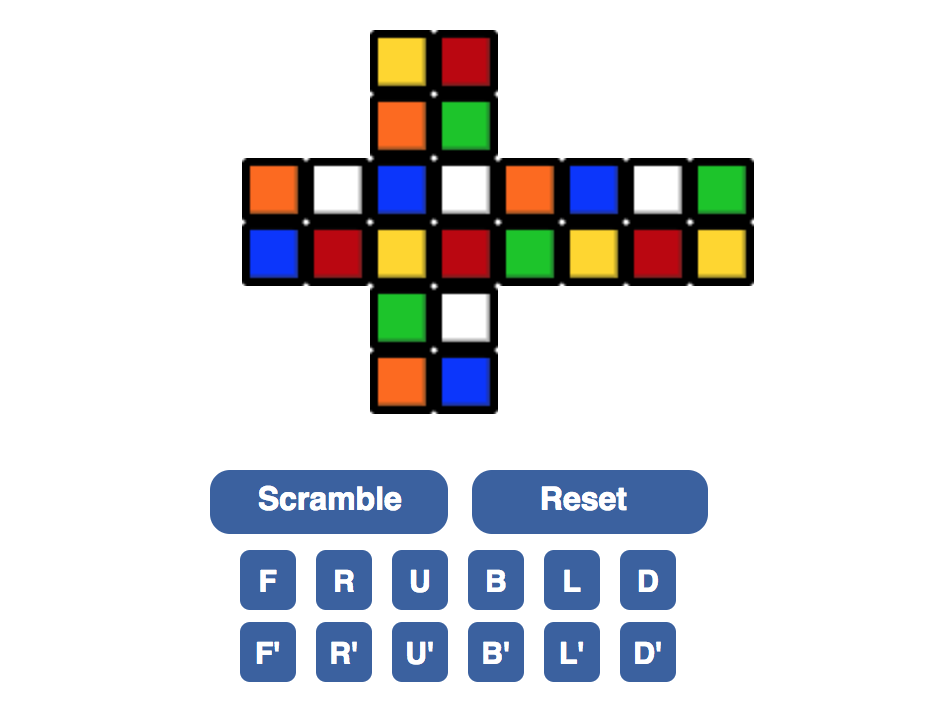
\includegraphics[width=\textwidth]{pics/2x2x2OnlineSim_Verification.png}
\end{subfigure}
\begin{subfigure}{.5\textwidth}
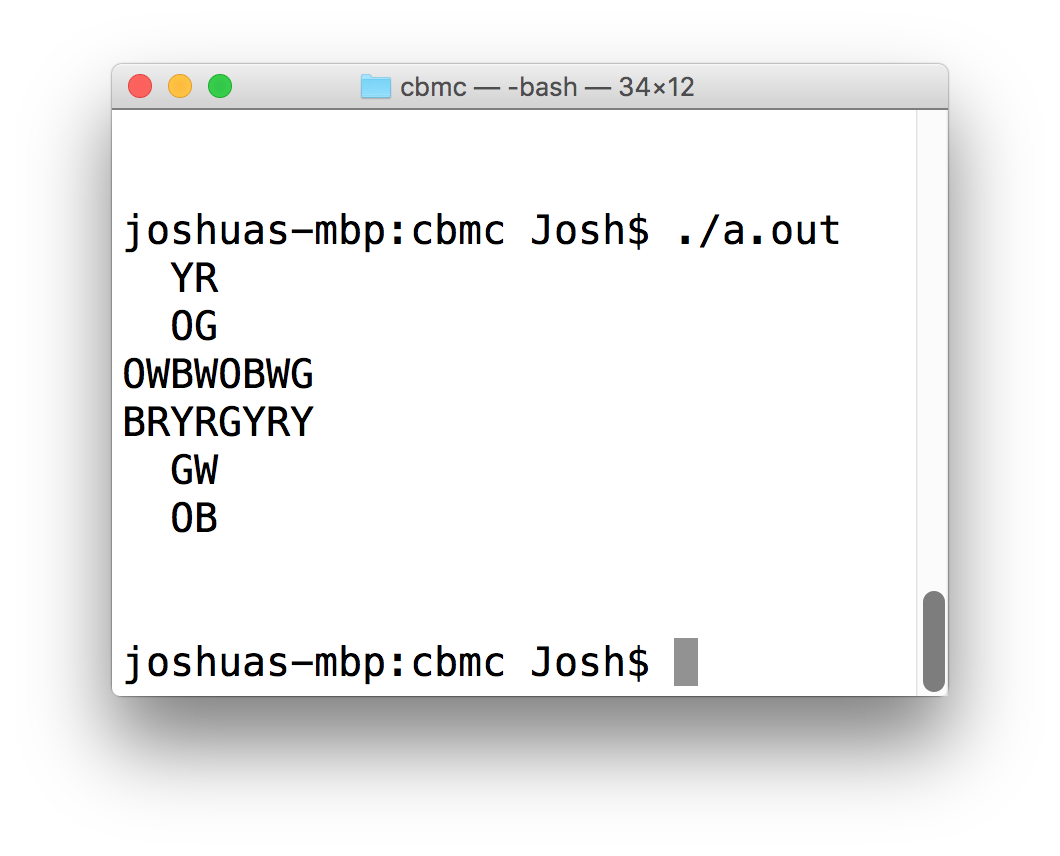
\includegraphics[width=\textwidth]{pics/2x2x2Sim_Verification.png}
\end{subfigure}
\caption{Comparing the move sequence 'FRUBLD'}
\end{figure}

\noindent Though simplistic, this method allowed quick elimination of simple errors (such as mis-numbering in the facelets or reversed faces in the adjacency list). After testing many sequences of rotation without apparent fault, it was determined that the transition relation (and the model itself) were correct representations of the cube.\\

\noindent Initially, upon completing the C model shown above, the goal was to return to the SMV model, so that nuXmv bounded model checking could be used to produce an answer. Unfortunately, this model was again difficult to capture. The primary issue was that the model seemed to grow overly complicated quite quickly, with the full state machine itself essentially being encoded. Upon this realization, the need for another model of the system was questioned. Instead, the C model itself may be used for model checking.

\subsection {C Bounded Model Checker (CBMC)}

The C Bounded Model Checker (CBMC) was first demonstrated by Clarke et al in 2004, as a way to check the consistency of Verilog and C models of hardware and software systems \cite{clarke}. By converting ANSI-C code into an intermediate, symbolic representation, the full program could be captured in CNF form and given to a SAT solver to verify conformance to a series of assertions. Through the use of a special set of functions to capture assumptions, assertions, and nondeterminism, CBMC is able to compute whether there exists a valid execution of a C program which violates the given properties. \\

\noindent To prepare the model for CBMC, a few additions were made to capture the notion of the ``final state" of the cube (see Appendix F). Though CBMC does provide command-line options for limiting the length of the search, as well as using built-in techniques to automatically do so (thus ``Bounded"), this model instead includes a natural bound as the result of a for-loop that runs only 14 times (see ``Background") and non-deterministically selects a move in each iteration. The target assertion (that the Rubik's cube is in the goal state) is then checked for each iteration. 


\subsubsection {CBMC Results}

Upon running CBMC, with the aforementioned assertions and assumptions, the result was a SAT query with the following specifications:

\begin{figure}[h]
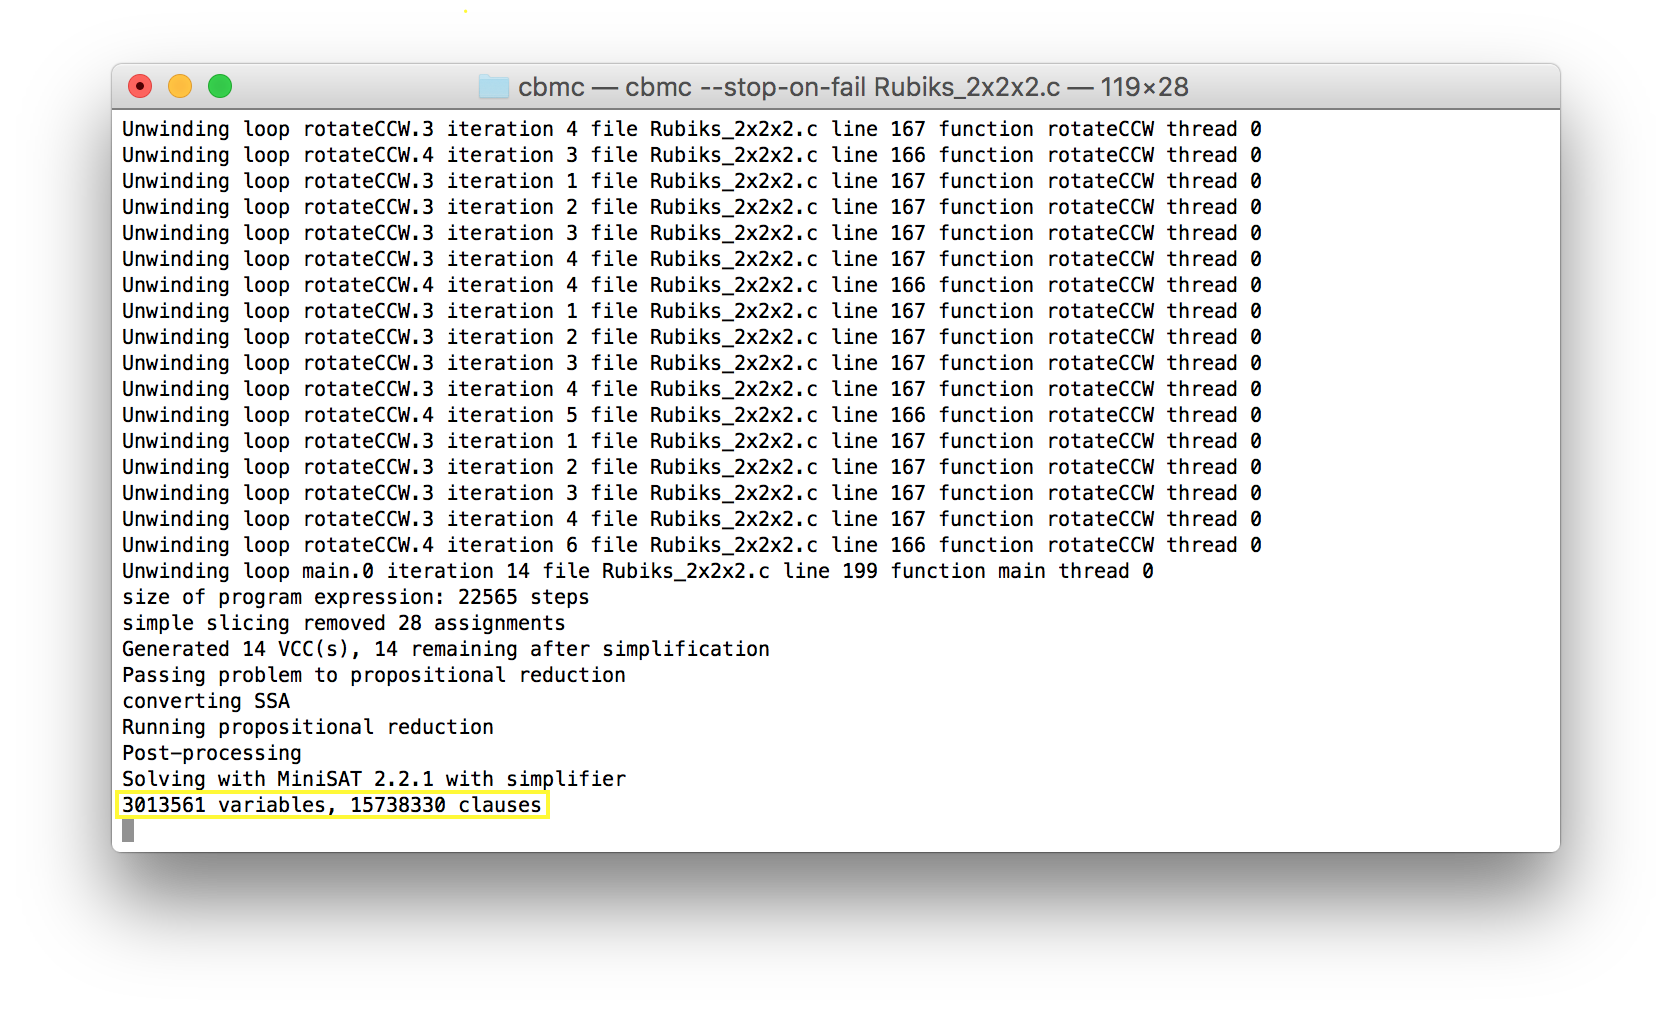
\includegraphics[width=\textwidth]{pics/2x2x2_SAT_Query_Specs.png}
\caption{SAT query specs for the move sequence `FRUBLD'}
\end{figure}

\noindent This model generated a drastically larger number of variables and clauses than the direct SAT method (via SABR) outlined above. However, the CBMC approach still produced results within a reasonable time ($\sim$450s).\\

\noindent The results of this model checking run included a counterexample trace that could be reduced to a list of moves for solving the cube. Upon receiving this list, the moves were performed on both the online and locally simulated cubes. In both cases, the set of moves was successfully able to solve the cube.

\begin{figure}[h]
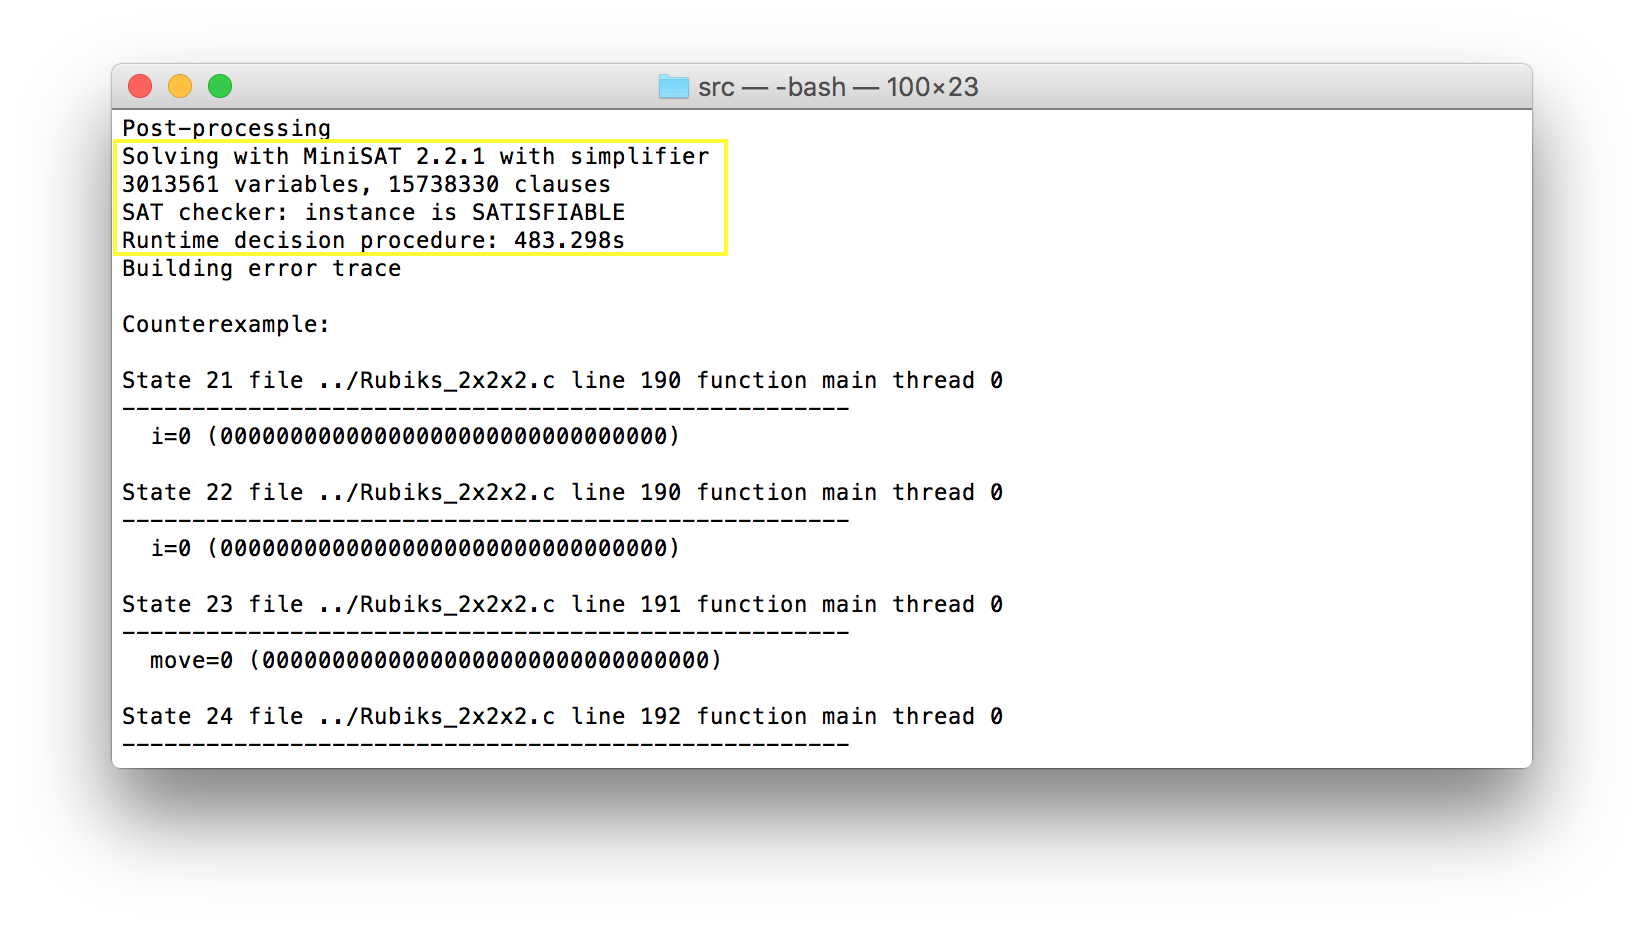
\includegraphics[width=\textwidth]{pics/2x2x2_Successful_Solve.png}
\caption{Model checking results for the move sequence `FRUBLD'}
\end{figure}

\noindent It should be noted that, should the reader choose to replicate the work given above, command line options were used with CBMC to ensure correctness. As a result of the way that the C model was written the for-loop would \textbf{always} run 16 times. Depending on the placement of the assertion, the results of the model checking run may be different:

\begin{enumerate}
\item If the assertion was placed within the for-loop, then the return counterexample may continue past the goal state to keep searching. This is as a result of the unrolling that occurs within CBMC. An assertion appearing within a loop is actually unrolled into a set of separate assertions, each of which is checked in the unrolled code. CBMC will continue searching until the end of the program is reached (i.e. all iterations of the loop are complete) or until all of the assertions have failed (in this case, necessarily until all iterations of the loop are complete). This is unnecessarily wasteful for the (significant) number of arrangements that are less than 16 rotations away.
\item If the assertion was placed outside of the for-loop, then, interestingly, the result is the search for a counterexample \textbf{of exactly a certain length}. In this case, for example, rather than checking for an example within 16 steps, CBMC would be searching for the target configuration after 16 moves have been nondeterministically selected and made.
\end{enumerate}

\noindent To counteract this issue, CBMC includes the ``--stop-on-fail" command line option. By placing the assertion within the for-loop, and using this option, the search will halt immediately upon finding a valid path to the violating state. This interesting contrast in results suggests that the model checking approach may be find optimal solutions through an iterative approach on the for-loop (by searching for a violation within 1 move, then 2 moves, etc.). Though on the surface this appears to be true, the actual resulting counterexample is longer than the sequence of moves used to reach the target state when creating the test case (`FRUBLD').\\

\noindent As mentioned previously, much of the verification effort was simply by inspection. The use of CBMC, however, provided for more chances to verify the correctness of the model. Perhaps the simplest check was to just try searching from different configurations. As discussed above in ``Background", it is proven that all configurations can be solved within 16 moves. As such, the lack of a counterexample for a given model checking run demonstrates that there is a flaw in the model, the asserted property, or the command line options used for CBMC. The presence of counterexamples for the tested configurations contributes towards an argument of correctness for the model. Additionally, other assertions may be made (such as checking for too many facelets of a single color, or incorrectly colored facelets along edges) to ensure that the model is correct.

\subsection {3x3x3 Model}

As the 2x2x2 model was successfully used to produce solutions, it was decided again that there was no need for an SMV model to perform the model checking run. Instead, again, a model in C with CBMC would be sufficient.

\subsubsection {C}

Unlike the case of the 2x2x2 model, the 3x3x3 model was quite simple to implement initially, taking less than an hour to create. By carefully placing the new cubes (`X5-8' for each side `X'), the adjacency list was easily extended to capture the transition relation for the 3x3x3. Again, an interactive version of the model was created first, so that it could be compared to existing implementations for correctness. This code is included in Appendix G.

\subsection {Verification}

Similar to the 2x2x2 verification effort, the first round simply consisted of inspecting correctness compared to an online simulator of the cube. Each individual rotation was checked, before checking a sequence of several rotations. Errors were corrected by printing the state of the cube after each rotation, in an attempt to locate at which point the transition relation had failed.\\

\noindent Again, this method revealed simple errors in the model. As an example, initially, some of the center facelets would move; given the transition relation intended, these facelets should remain stationary regardless of the rotations occurring around them. The transition relation was appropriately fixed to prevent this from happening. \\

\begin{figure}[h]
\begin{subfigure}{.5\textwidth}
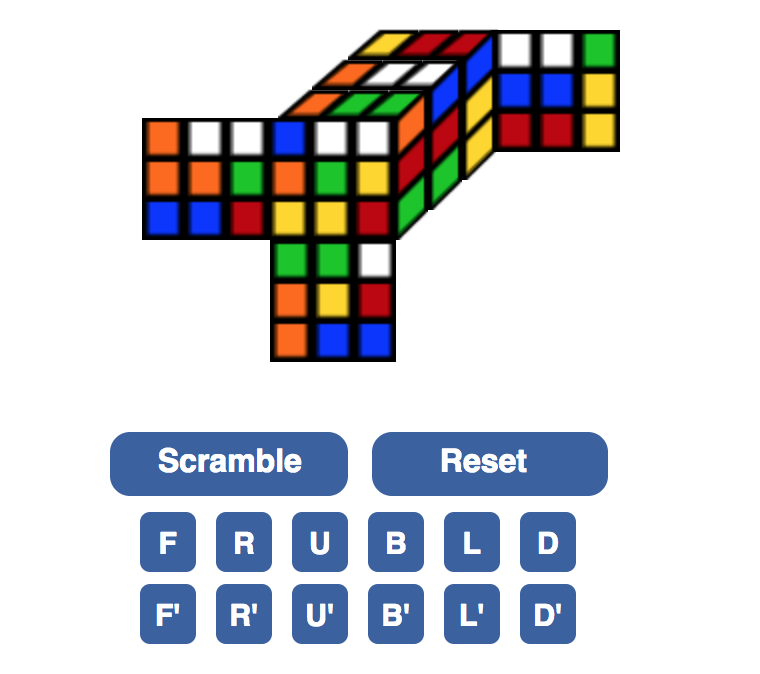
\includegraphics[width=\textwidth]{pics/3x3x3OnlineSim_Verification.png}
\end{subfigure}
\begin{subfigure}{.5\textwidth}
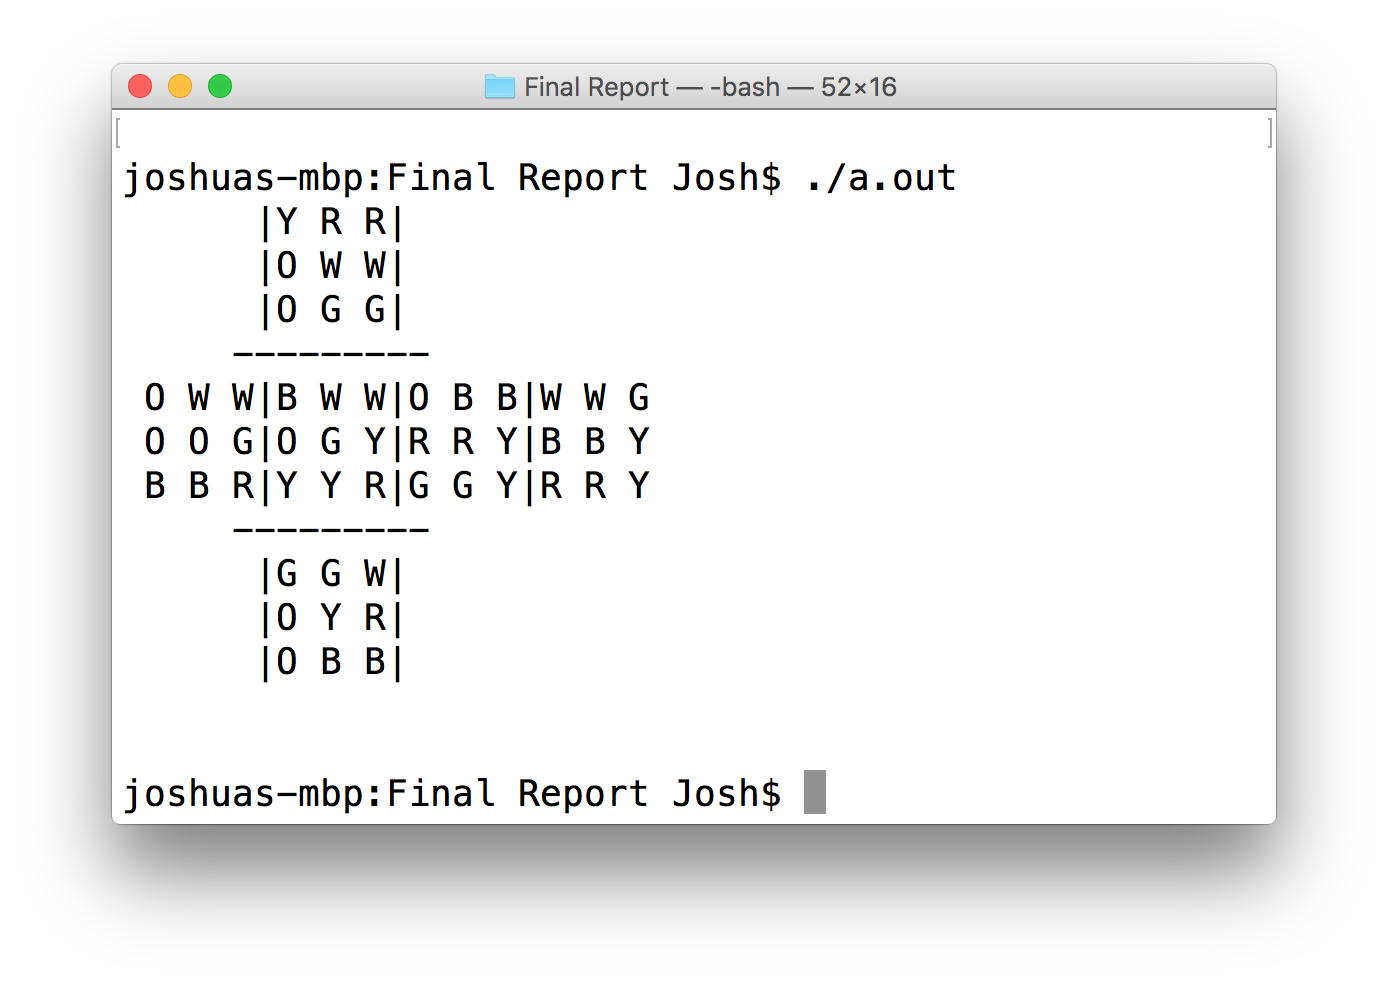
\includegraphics[width=\textwidth]{pics/3x3x3Sim_Verification.png}
\end{subfigure}
\caption{Comparing the move sequence 'FRUBLD'}
\end{figure}

\noindent Due to the structure of a 3x3x3 Rubik's Cube, a 2x2x2 cube may be simulated by simply disregarding the center and edge (but not corner) cubes. As a result of this property, an additional verification step was to perform the series of moves found in the first model checking run on both the online and locally simulated cubes. The result should be that the corner cubes appear solved (though the remaining cubes do not).

\subsection {Initial CBMC Results}

Again, the C model was appropriately annotated (see Appendix H) to allow for CBMC to locate a counterexample trace. It should be noted that, for a 3x3x3 cube, God's Number is 26 quarter turns. As a result, the for-loop is appropriately changed to account for this. CBMC was then run on this model, in the pursuit of an appropriate counterexample trace. Unfortunately, the conversion of this model to a SAT query was much less successful (see Figure 7).\\

\noindent Given the significant number of variables ($\sim$17 million) and clauses ($\sim$93 million) generated by CBMC, a solution was incalculable within any reasonable amount of time. In order for this method to be useful, a closer look was, and still is, needed at the inner workings of CBMC and Minisat, the underlying SAT solver called by the model checker.\\

\begin{figure}[h]
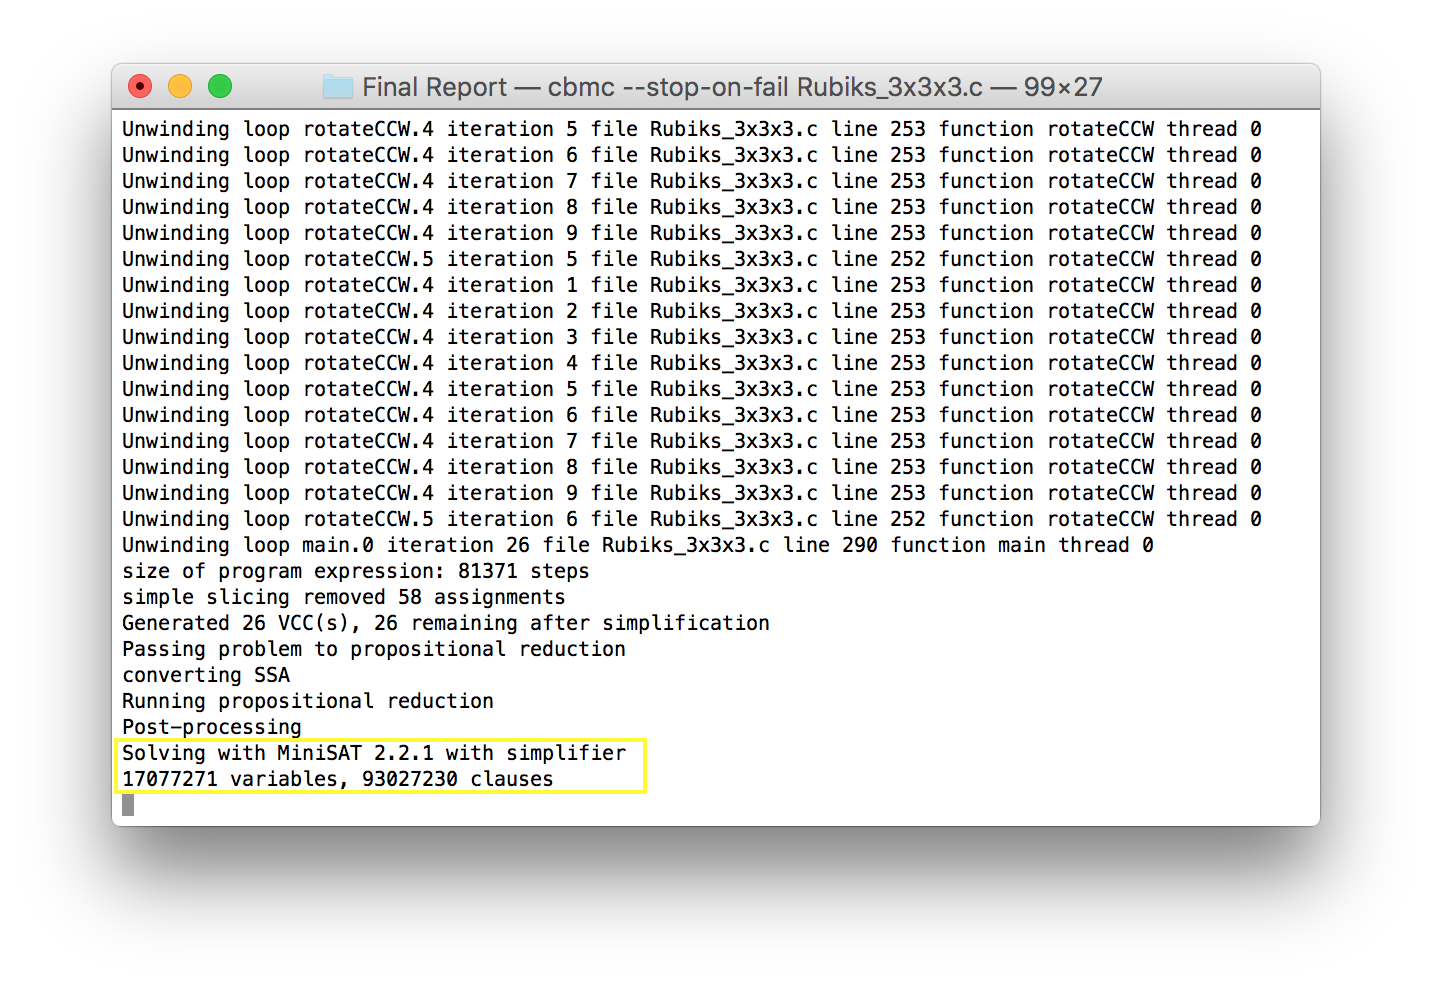
\includegraphics[width=\textwidth]{pics/3x3x3_SAT_Query_Specs.png}
\caption{Initial SAT query specs for the move sequence `FRUBLD'}
\end{figure}

\subsection {``Under the hood": Minisat and CBMC}

In pursuit of answers as to what optimizations might be made to the 3x3x3 model, the original papers for Minisat \cite{een} and CBMC \cite{clarke}, \cite{clarke2} were consulted. Upon reviewing the CBMC paper, it was clear that the conversion heavily favored unrolled loops, an absence of pointers, and the avoidance of arrays. For pointers, the number of CNF clauses and variables grew exponentially, as a clause was generated to represent not only the actual assignment of the pointer given in the code, but also for every possible assignment based on the given datatype. Similarly, assignments to array variables generated a significant number of additional variables and clauses, to capture not only that an assignment had been made to the correct cell, but also that no assignments had been made to the other cells. Finally, loop unrolling required a series of intermediate steps, creating several GOTO statements and conditionals. \\

\noindent The authors of Minisat were also very transparent in the workings of their software. Minisat was designed to be intentionally clear and simple to interested developers, but was also meant to be general in the set of problems for which it is applicable. As such, several of the heuristics are not necessarily tuned to solve Rubik's Cubes. While the exact effects on this problem were not studied closely for this work, fine-tuning of multiple constants used within the source code of Minisat could improve overall performance. For example, Minisat disregards learned clauses after they go unused for a certain amount of time. It is possible that, in the case of this particular problem, these learned clauses may be valuable, and the constant could be adjusted appropriately (at the cost of memory during the software execution).

\subsection {Revised 3x3x3 C Model \& Final CBMC Results}

To compensate for the potential sources of overhead mentioned above, the 3x3x3 model was modified to be as amenable to CNF translation as possible: all loops were unrolled, all pointers were eliminated, and all arrays were turned into individual, disconnected variables. As well, the number of function calls was reduced (as this generated additional statements in the form of GOTOs in the CNF conversion). The result was a significantly larger model (included in the repository for this project). As expected, upon running CBMC on the new model, drastically better results were observed:\\

\begin{figure}[h]
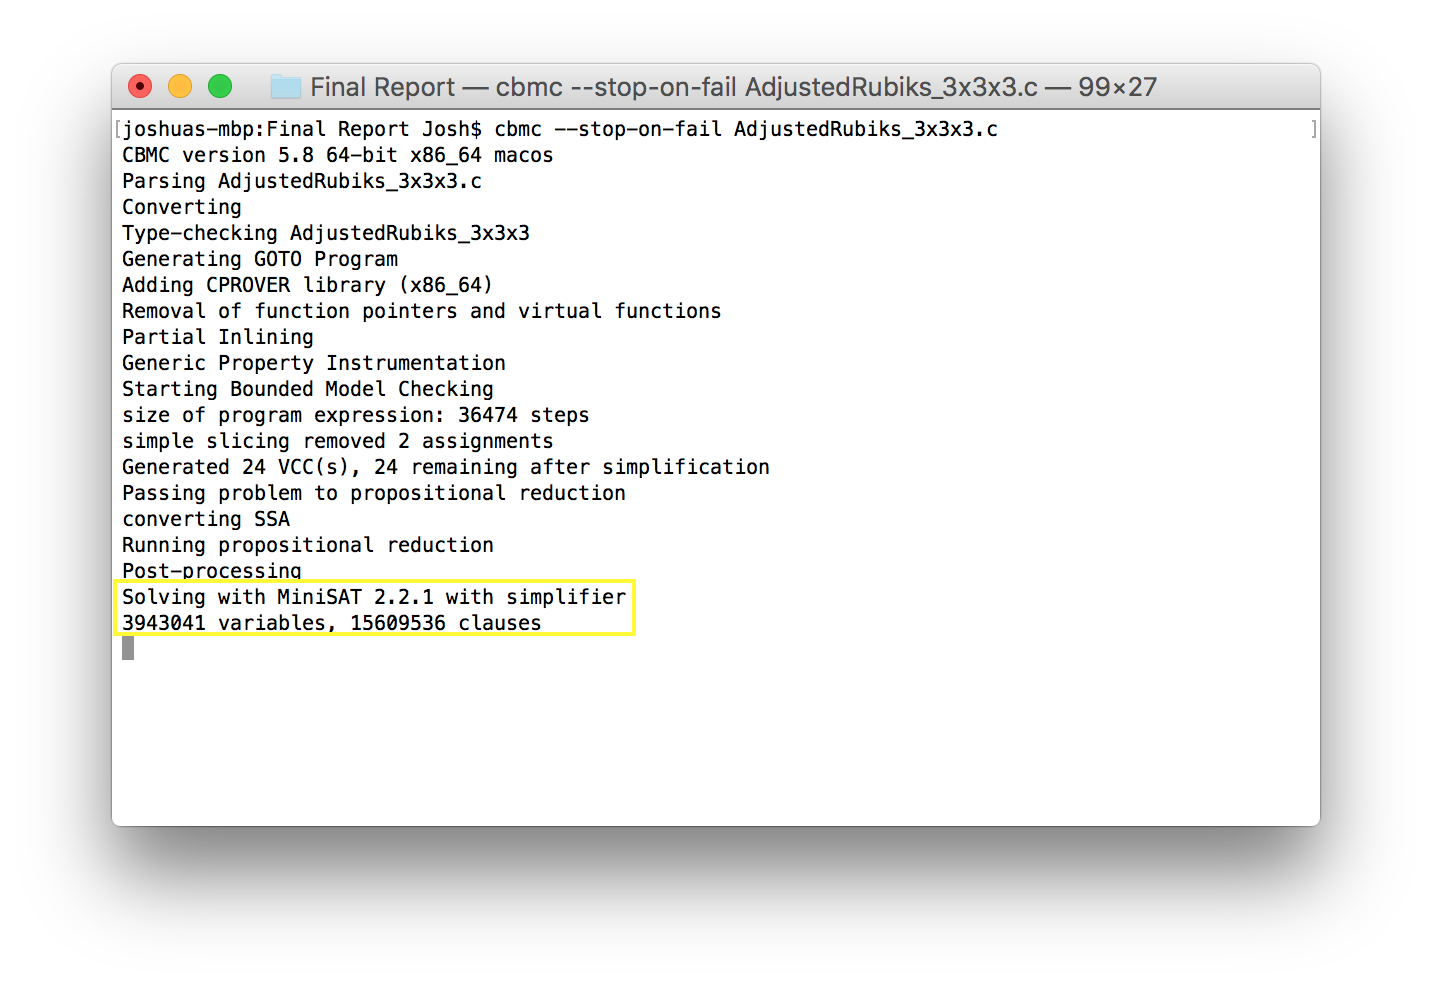
\includegraphics[width=\textwidth]{pics/3x3x3Adjusted_SAT_Query_Specs.png}
\caption{Adjusted SAT query specs for the move sequence `FRUBLD'}
\end{figure}

\noindent Unfortunately, though the number of variables was reduced by a factor of nearly 4 and the number of clauses by a factor of nearly 6, the reduction was not sufficient to produce a solution within a reasonable amount of time. This was somewhat shocking as the number of variables and clauses was on par with that of the 2x2x2 Rubik's Cube model checking instance. The likely cause of this discrepancy may be either the lack of fine-tuning for Minisat and CBMC, or because the complexity of the generated clauses is such that a solution cannot be computed as quickly. \\

\noindent One final adjustment to the 3x3x3 model was made (with the modified source available in the repository for this project), in order to see what effect it would have on the computation. Rather than unrolling every loop for the model, the loop in main was left as it appeared in the original version of the model. CBMC was then run on this model to check for a solution:\\

\begin{figure}[h]
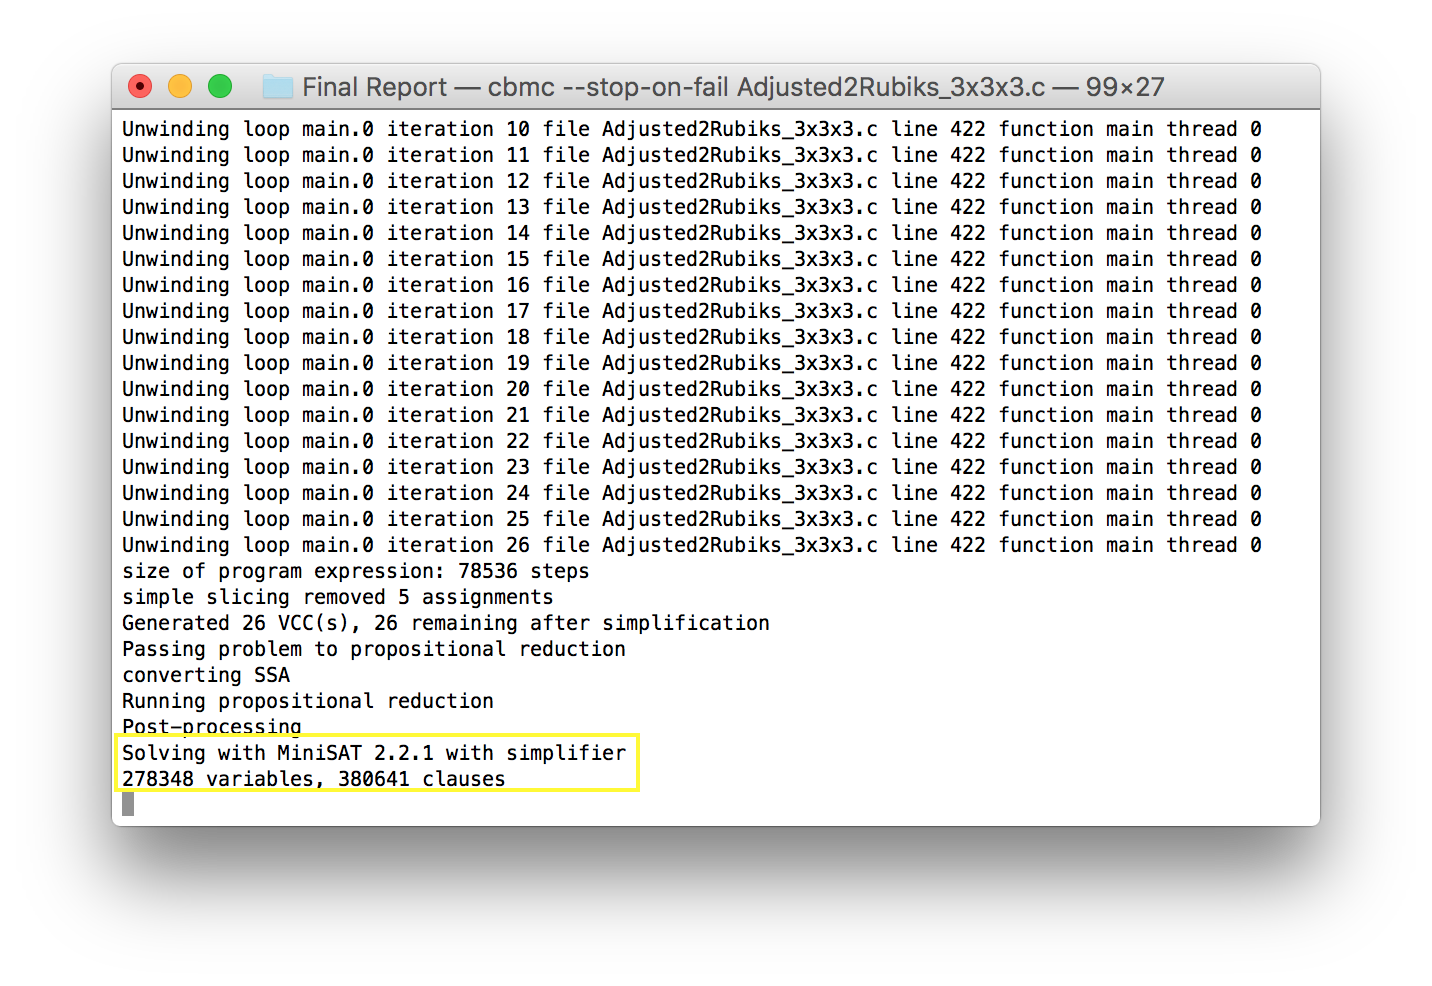
\includegraphics[width=\textwidth]{pics/3x3x3Adjusted2_SAT_Query_Specs.png}
\caption{Second Adjusted SAT query specs for the move sequence `FRUBLD'}
\end{figure}

\noindent Unexpectedly, the number of variables and clauses was reduced even further. This placed the SAT query for the 3x3x3 within two orders of magnitude of the SABR query generated above. That being said, a solution was still not computed in sufficient time. Again, it is possible that tool optimizations, the lack of model optimizations, and/or the complexity of the generated CNF clauses are to blame.

\subsection {Conclusion \& Future Work}

Though, initially, SMV seemed like an appropriate modeling language for this problem, the actual act of modeling proved to be to complicated and difficult to bug. Alternatively, using C proved to be relatively straightforward. This approach may have simply shifted the focus from developing a correct model (as was the issue in SMV) to instead optimizing a correct model (as was the issue in C). Either way, the final C model proved to be very effective for a 2x2x2 Rubik's Cube, producing a solution in approximately seven minutes, while it was not appropriate for a 3x3x3 cube. The attempts made at optimizing code significantly reduced the size of the SAT query generated for the problem, but still the query proved to be too large for the machine used to produce a solution within reasonable time.\\

\noindent As discussed previously, the code for both CBMC and Minisat are publicly available, with scholarly works discussing how exactly each works. Future attempts at using a bounded model checking approach for solving Rubik's Cubes may need to focus on optimizing each of these tools appropriately for the problem. A thorough comparison of the generated SAT queries by SABR and CBMC might provide a hint as to how exactly the CBMC ANSI-C conversion could be further improved. Study of the heuristics used in Minisat, as well as the learning process used, could indicate how numeric constants and algorithms could be altered. Additionally, the work on SAT solver development included in the Minisat paper provides 
sufficient information such that a specialized ``RubikSAT" could be developed specifically to solve this problem.

\section{Final Conclusions}
With all the results and conclusions made about each method described above in mind there are some conclusions that can be made about this study. Overall, the SAT solving technique appears to make the most sense for solving a Rubik’s cube. However, this difficulty in getting a SAT solver to solve a 3x3 Rubik’s cube in a reasonable amount of time indicates that some optimizations within the SAT solver itself needs to be done to make this method practical. The spin method of solving the Rubik’s cube provides an interesting deviation from the tradition SAT solving method and with more development could lead to quicker runtimes and a more adaptable model. In general, using the Sabr language and the provided infrastructure makes solving puzzle-like problems a breeze and with a few tweaks could provide an almost perfect solution to the problem discussed in this study.

\pagebreak
\begin{center}
Appendix A
\end{center}

\begin{center}
Table 1. Extended miniSat 2x2 Rubik's cube results \\[1mm]
\end{center}
\begin{adjustwidth}{-3.5cm}{}
\begin{tabular}{|c|c|c|c|c|c|c|c|c|c|}
\hline
Run Number & SAT & Parse time & Restarts & Conflicts /sec & Decisions /sec & Conflict literals & Memory used & CPU time \\
\hline
0 & Y & 0.01 s & 307 & 24015 & 42318 & 16.40\% deleted & 18.83 MB & 4.776 s \\
\hline
1 & Y & 0.01 s & 1341 & 21611 & 32719 & 15.89\% deleted & 25.42 MB & 29.368 s \\
\hline
2 & N & 0.01 s & 1532 & 24952 & 37551 & 23.72\% deleted & 24.79 MB & 28.036 s \\
\hline
3 & Y & 0.01 s & 2044 & 20364 & 30679 & 18.07\% deleted &  26.29 MB & 46.368 s \\
\hline
4 & Y & 0.01 s & 24574 & 13853 & 18578 & 35.33\% deleted & 80.81 MB & 1186.84 s \\
\hline
5 & Y & 0.01 s & 236 & 26659 & 44732 & 13.62\% deleted & 12.32 MB & 2.812 s \\
\hline
\end{tabular} \\[3mm]
\end{adjustwidth}

\begin{center}
Table 2. Extended CaDiCaL 2x2 Rubik's cube results \\[1mm]
\end{center}
\begin{adjustwidth}{-3.5cm}{}
\begin{tabular}{|c|c|c|c|c|c|c|c|c|c|}
\hline
Run Number & SAT & Parse time & Restarts & Conflicts /sec & Decisions /sec & Conflict literals & Memory used & CPU time \\
\hline
0 & Y & 0.01 s & 9813 & 390697 & 11103.13 & 7.63\% deleted & 15.67 MB & 35.67 s \\
\hline
1 & Y & 0.01 s & 4693 & 13438.41 & 53381.47 & 7.35\% deleted & 9.10 MB & 11.59 s \\
\hline
2 & N & 0.01 s & 3167 & 16655.43 & 57761.16 & 7.81\% deleted & 8.47 MB & 7.89 s \\
\hline
3 & Y & 0.01 s & 29175 & 5824.01 & 21442.38 & 11.11\% deleted & 21.96 MB & 160.65 s \\
\hline
4 & Y & 0.01 s & NA & NA & NA & NA & NA & $\>$ 20000 s \\
\hline
5 & Y & 0.01 s & 2172 & 18536.71 & 74321.68 & 6.05\% deleted & 6.77 MB & 4.00 s \\
\hline
\end{tabular}
\end{adjustwidth}

\pagebreak
\begin{center}
Appendix B
\end{center}
\lstinputlisting[language=Promela]{sivets_model.pml}

\begin{center}
Sabr 3x3 Rubik's Cube model
\end{center}
\begin{lstlisting}
# SABR
# solve 3x3 rubiks cube

Sym{ b o w r g y }

Board{
.....		b1 b2 b3;
.....		b4 .  b6;
.....		b7 b8 b9;
r1 r2 r3	y1 y2 y3 	o1 o2 o3	w1 w2 w3;
r4 .  r6	y4 .  y6 	o4 .  o6	w4 .  w6;
r7 r8 r9	y7 y8 y9 	o7 o8 o9	w7 w8 w9;
.....		g1 g2 g3;
.....		g4 .  g6;
.....		g7 g8 g9;
}

Start{
		y g b;
		g	g;
		o b w;
r o g	w r b	o y y	o r b;
b	w	o	b	y	b	o	w;
b w w	b y g	y r g	r o r;
		r r o;
		g	w;
		w y y;
}

End{
		b b b;
		b   b;
		b b b;
r r r	y y y 		o o o	w w w;
r   r	y   y 		o   o	w	w;
r r r	y y y 		o o o	w w w;
		g g g;
		g   g;
		g g g;
}

Trans Clock:Side{

	t1 t2 t3;

l3	f1 f2 f3	r1;
l2	f4    f6	r2;
l1	f7 f8 f9	r3;

	b1 b2 b3;
=>
	l1 l2 l3;

b1	f7 f4 f1	t1;
b2	f8    f2	t2;
b3	f9 f6 f3	t3;

	r3 r2 r1;
}

Trans CounterClock:Side{

	t1 t2 t3;

l3	f1 f2 f3	r1;
l2	f4    f6	r2;
l1	f7 f8 f9	r3;

	b1 b2 b3;
=>
	r1 r2 r3;

t3	f3 f6 f9	b3;
t2	f2    f8	b2;
t1	f1 f4 f7	b1;

	l3 l2 l1;
}

DesObj Front:Side{
	b7 b8 b9;
	
r3	y1 y2 y3	o1;
r6	y4    y6	o4;
r9	y7 y8 y9	o7;
	
	g1 g2 g3;
}

DesObj Top:Side{
	w3 w2 w1;

r1	b1 b2 b3	o3;
r2	b4    b6	o2;
r3	b7 b8 b9	o1;

	y1 y2 y3;
}

DesObj Back:Side{
	b3 b2 b1;

o3	w1 w2 w3	r1;
o6	w4    w6	r4;
o9	w7 w8 w9	r6;

	g8 g7 g6;
}

DesObj Bottom:Side{
	y7 y8 y9;

r9	g1 g2 g3	o7;
r8	g4    g6	o8;
r7	g7 g8 g9	o9;

	w9 w8 w7;
}

DesObj Left:Side{
	b1 b4 b7;

w3	r1 r2 r3	y1;
w6	r4    r6	y4;
w9	r7 r8 r9	y7;

	g7 g4 g1;
}

DesObj Right:Side{
	b9 b6 b3;

y3	o1 o2 o3	w1;
y6	o4    o6	w4;
y9	o7 o8 o9	w7;

	g3 g6 g9;
}
\end{lstlisting}

\newpage

\begin{center}
Appendix D: Initial 2x2x2 SMV Model
\end{center}

\lstinputlisting[language=Promela]{RubiksCube_2x2x2.smv}

\newpage

\begin{center}
Appendix E: 2x2x2 C Model
\end{center}

\lstinputlisting[language=C]{Rubiks_2x2x2_Interactive.c}

\newpage

\begin{center}
Appendix F: CBMC Annotated 2x2x2 C Model
\end{center}

\lstinputlisting[language=C]{Rubiks_2x2x2.c}

\newpage

\begin{center}
Appendix G: 3x3x3 C Model
\end{center}

\lstinputlisting[language=C]{Rubiks_3x3x3_Interactive.c}

\newpage

\begin{center}
Appendix H: CBMC Annotated 3x3x3 C Model
\end{center}

\lstinputlisting[language=C]{Rubiks_3x3x3.c}

\newpage

\begin{thebibliography}{9}

\item{2DSim}
\textit{Online 2D Pocket Cube Simulator}. https://ruwix.com/online-puzzle-simulators/2x2x2-pocket-cube-simulator.php.

\item{3DSim}
\textit{Online 3D Rubik's Cube Simulator}. https://ruwix.com/online-puzzle-simulators/3x3x3-rubiks-cube-simulator.php.

\bibitem{biere} Biere, A. et al. ``Bounded Model Checking." \textit{Advances in Computers}, vol. 58, 2003.

\bibitem{CaDiCaL} 
\textit{{CaDiCaL}. 
http://fmv.jku.at/cadical/}

\bibitem{cbmc} \textit{The C Bounded Model Checker (CBMC)}. http://www.cprover.org/cbmc/.

\bibitem{chenjingchao} 
Chen, Jingchao. 
\textit{{Solving Rubik's Cube Using SAT Solver}. 
Computing Research Repository - CORR, 2011.}

\bibitem{clarke} Clarke, E. , Kroening, D. and Yorav, K. 2003. ``Behavioral consistency of C and verilog programs using bounded model checking." In \textit{Proceedings of the 40th annual Design Automation Conference (DAC '03)}. ACM, New York, NY.

\bibitem{clarke2} Clarke, E., Kroening, D., Sharygina, N. et al. Formal Methods in System Design (2004) 25: 105. 

\bibitem{een} Een N., Sorensson N. (2004) An Extensible SAT-solver. In \textit{Theory and Applications of Satisfiability Testing}. SAT 2003. Lecture Notes in Computer Science, vol 2919.

\bibitem{nuxmv}
\textit{nuXmv Model Checker}. https://nuxmv.fbk.eu/. 

\bibitem{sabr} 
\textit{{Sabr}. 
http://sabrlang.org/}

\bibitem{satrubiks}
SatRubiks.
\textit{{Github repository}.
https://github.com/IowaStateAerospaceCourses-Rozier/final-project-satrubiks}
\end{thebibliography}

\end{document}
